\documentclass{article}
\usepackage{color}
\usepackage{listings}
\usepackage{graphicx}
\lstset{ %
language=java,                % choose the language of the code
basicstyle=\footnotesize,       % the size of the fonts that are used for the code
numbers=left,                   % where to put the line-numbers
numberstyle=\footnotesize,      % the size of the fonts that are used for the line-numbers
stepnumber=1,                   % the step between two line-numbers. If it is 1 each line will be numbered
numbersep=5pt,                  % how far the line-numbers are from the code
backgroundcolor=\color{white},  % choose the background color. You must add \usepackage{color}
showspaces=false,               % show spaces adding particular underscores
showstringspaces=false,         % underline spaces within strings
showtabs=false,                 % show tabs within strings adding particular underscores
frame=single,           % adds a frame around the code
tabsize=2,          % sets default tabsize to 2 spaces
captionpos=b,           % sets the caption-position to bottom
breaklines=true,        % sets automatic line breaking
breakatwhitespace=false,    % sets if automatic breaks should only happen at whitespace
escapeinside={\%*}{*)}          % if you want to add a comment within your code
}
\begin{document}
\tableofcontents{}


\newpage
\section{Einführung}
Performanz spielt eine große Rolle in der Entwicklung von Hardware. Um herauszufinden ob die Hardware performant genug ist, werden Workloads
verwendet um die Grenzen der Hardware zu testen. Aber auch nicht nur Hardware, sondern Virtuelle Maschinen können getestet werden, 
wo virtuelle CPUs oder der Hypervisor getestet werden. [2]
Sowie in Cloud Computing können solche Tests durchgeführt werden [3]. Somit gibt es ein weites Spektrum an Auswahl, wo solche Tests wichtig sind.
\textit{Die Performanz eines Systems kann dabei sowohl durch Probleme in der Soft-
ware, CPU-Zeit oder andere Hardwareressourcen begrenzt werden. Durch die standar-
disierten Benchmarks wird es möglich, die Performanz verschiedener Hardware- und
Softwareanbieter zu vergleichen.}

Die größten Probleme in den Großkonzernen sind Performanzprobleme und nicht die funktionellen Probleme. Service Ausfälle kosten sind höchst kostspielig. 
Deshalb werden in High Performance Computing viele Tests durchgeführt, um ihre Grenzen zu analysieren [1].
In meiner Arbeit werde ich mit dem fio Tool arbeiten, um solche Performanzänderungen zu berechnen und zu analysieren.
Fio (flexible I/O Generator) ist ein Tool mit der man die Hardware-Performanz testen kann, z.B die Brandweite beim Schreiben einer Datei, und diesen Performanz-Test als log Daten ausgeben kann.
Mein Programm wird mit diesen Logs arbeiten, um mit ihnen besser arbeiten zu können oder auch besser darzustellen.
Ziel meines Tools soll es sein, dass man den stationären Zustand analysiert. 


\section{Grundlagen}
Mit dem Fio , kann man die Performanz auf einer bestimmten Hardware testen. I/O Geschwindigkeit wird in hier KiByte/Sekunde angegeben. 

fio besitzt kein GUI sondern arbeitet nur in der Konsole. Man kann für das Programm fio-Dateien schreiben oder auch in der Konsole arbeiten,
um seine gewünschten Task zu testen,
wie random read/write auf einer Datei.
Wenn man ein Random Read testen möchte, kann die fio-Datei so aussehen.
\newline
\begin{lstlisting}
    ; fio-rand-read.job for fiotest

    [global]
    name=rand-read # Name des Jobs
    rw=randread # Was soll der Job testen, randread = random read
    runtime=2s # Wie lange soll der Job laufen
    size=2m # Groesse der Datei, m fuer Megabyte
    write_bw_log=mytest # Name der Log-Datei
\end{lstlisting}
\bigskip
In der Konsole gebt man sie als Parameter an, wenn es nur ein schneller Test sein soll. Zusätzlich können die Tests, 
oder auch Jobs genannt, Logs ausgeben. Mit diesen Logs wird mein Tool arbeiten. Dieser Job oben testet das Random-Read mit einer
runtime von 2 Sekunden. Nun möchte man wissen, wann der stationäre Zustand erreicht wurde, wenn man solche Tests länger durchlaufen lässt.
Der stationäre Zustand ist der Zeitpunkt, wenn es keine starken Schwankungen mehr bei der Brandweite im Lesen und Schreiben gibt.
Das Schreiben und Lesen verhält sich außerdem nicht deterministisch. Das bedeutet, auch wenn man die selbe Datei mit dem Selben Computer lesen/schreiben
würde, wäre die Brandbreitengeschwindigkeit immer im Durchschnitt unterschiedlich. Weitere nicht deterministische Zustände könnte sogar CPU Temperatur sein,
oder CPU Scaling, parallele Prozessierung [SOURCE]. In Zukunft soll das Programm diese mit der Standardabweichung selber ausrechnen. 

Die Geschwindigkeit der Brandbreite ist abhängig von der CPU und des Speichermediums, wie SATA HDD, SATA SSD oder NVMe.
The main data created by our experiment is the time taken by each in-process iteration to run.
Formally, this is time series data of length 2000. In this Section we explain how we use statistical
changepoint analysis to enable us to understand this time series data and classify the results we
see, giving the first automated method for identifying warmup.
\textit{NVMe drives are expected to be widely adopted in datacenters}.
Warmup iterations
are intended to bring the JVM into a steady state (e.g., exe-
cute all applicable just-in-time compilations).


\section{Konzept}
Mein Tool soll mit den Logs vom fio Tool arbeiten. \newline
fio besitzt ein extra Parameter, um solche Workloads als log ausgeben zukönnen.
Workloads oder auch Jobs, sind die Performanz Tests die mit dem fio gemacht werden.
Für diese Workload möchte man noch gerne was eigentlich für Werte Zustande kamen.
Die Logdatei besitzt die Information. Sie besitzt die Information vom verlauf des Jobs in Millisekunden.
Die jeweils 5 Werte besitzen und mit Kommas getrennt sind.
Mit dem Parameter $write\_bw\_logs=[Dateiname]$, kriege ich diese Logdatei:
\begin{lstlisting}
    \[Time,	Bandwidth,	data direction, Blocksize,	Offset\]
    0, 	    59782, 		0,		        4096,		0
\end{lstlisting}
Time für die Zeit in Millisekunden (ms) die verlaufen ist, Bandwidth für die Brandweite in KiByte/s
Dritter Wert für die Date direction ob gelesen (= 0) oder geschrieben (= 1) wurde ein Blocksize
und ein Offset. Die Logdaten selbst sind immens lang und nicht schön lesbar. Deshalb wurde schon ein kleines Tool in Python gebaut 
was diese Logdaten zu einem Graph umwandelt. 
Die Y-Achse ist die Brandbreitengeschwindigkeit und X-Achse ist die vergangene Zeit des jeweiligen Jobs.
Wenn man die Logdaten anschaut, sieht man, dass die Brandbreitengeschwindigkeit sich schneller innerhalb einer 1 ms ändert.
\newpage
\begin{lstlisting}
    \[Time,	Bandwidth,	data direction, Blocksize,	Offset\]
    23, 	    59782, 		0,		        4096,		0
    23, 	    43534, 		0,		        4096,		0
    23, 	    54364, 		0,		        4096,		0

    X: 23       Y: 59782   ->        X: 23.0     Y: 59782
    X: 23       Y: 43534   ->        X: 23.3     Y: 59782
    X: 23       Y: 54364   ->        X: 23.6     Y: 59782
\end{lstlisting}
Da man die Daten nicht verwerfen möchte, wurden Wiederholungen linear getrennt. 
Für Veranschaulichung wurde das fio Tool auf meinem Rechner getestet mit dem
Command die oben erwähnt wurde. Die logdatei wurde ausgewertet und hier als .svg Datei dargestellt:
\\
\begin{figure}[ht!]
    \centering
    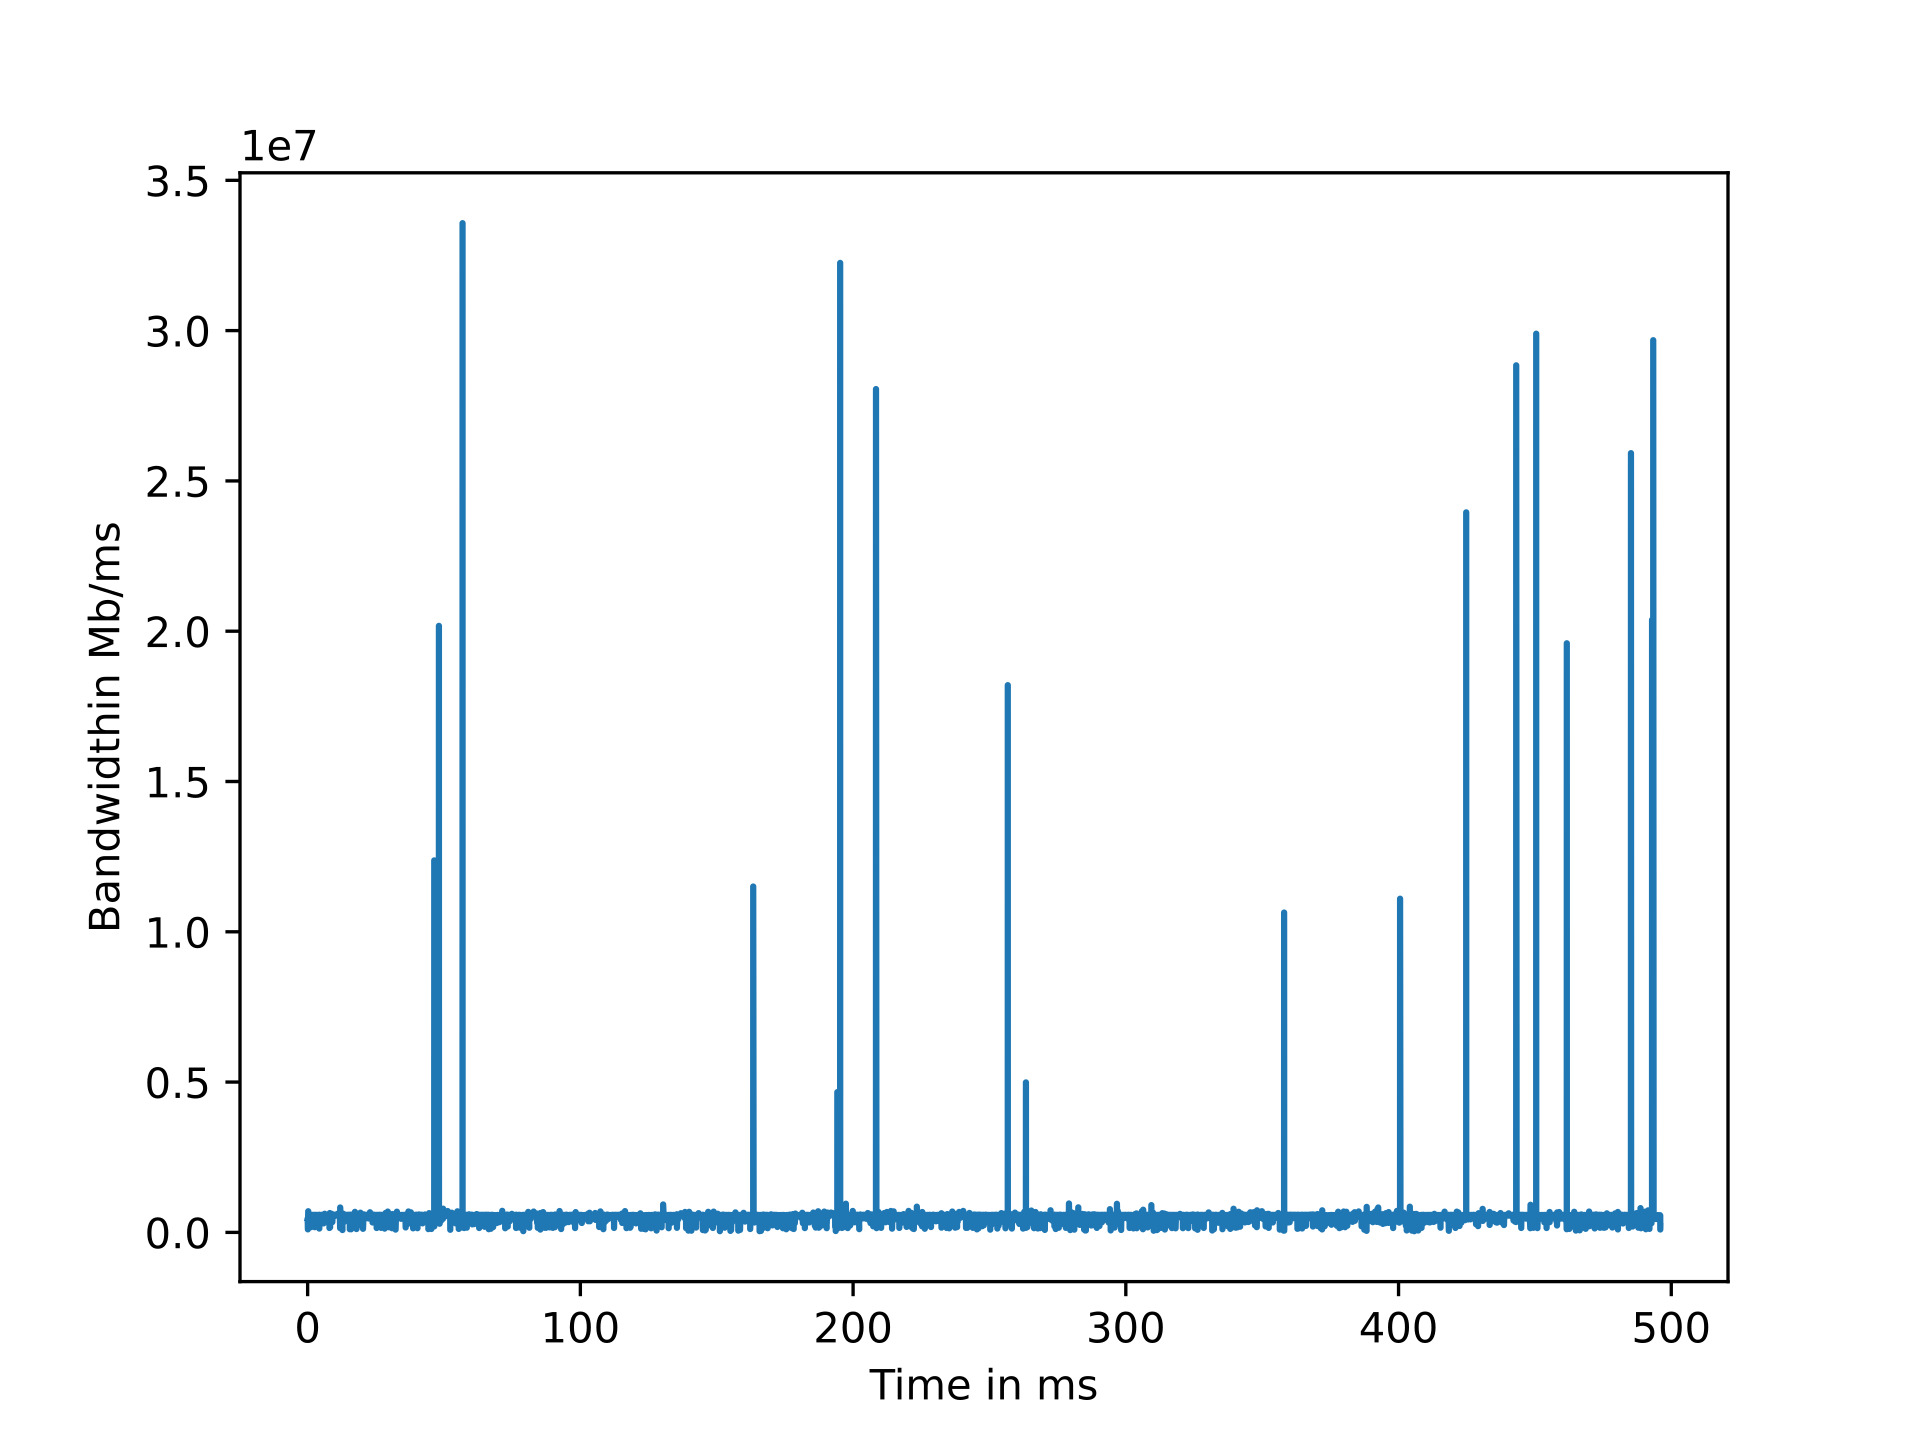
\includegraphics[width=120mm]{./Code/nm_mytest_bw.jpg}
    \caption{Plot tool Ausgabe mit Log Datei  \label{overflow}}
\end{figure}
Der Computer hat ein 11th Gen Intel(R) Core(TM) i5-11400 @ 2.60GHz und eine ADATA SWORDFISH SSD als Datenträger.
Es wurde ein kleines Tool geschrieben. Die eigentliche Arbeit wird es sein, das Tool weiter auszubauen das nicht nur veranschaulicht
sondern auch den stationären Zustand berechnet. Das Programm wird in Java geschrieben. Grund dafür ist, da dort die bereits die meiste Erfahrung steckt.
Eine Möglichkeit, den stationären Zustand zu ermitteln, wäre das man die Standardabweichung verwendet und errechnet, wann die Abweichung klein ist.
\textit{With improvements in storage device technology, the once negligible cost of I/O stack time has become more relevant (Foong et al. 2010; Caulfield et al. 2010). A number
of studies have provided proof of the I/O software stack being the major performance bottleneck in future storage systems.}
\section{Verwandte Arbeiten}
\section{Zeitplan}
\section{Referenz}
\begin{itemize}
    \item An Automated Approach for Recommending When to Stop Performance Tests [1]
    \item Virtual Machine Performance Analysis and Prediction [2]
    \item A Comparative Study of High-Performance Computing on the Cloud [3]
    \item A Case for High Performance Computing with Virtual Machines [4]
\end{itemize}
\end{document}